\chapter{相关技术及理论}
本章将概述短文本分类问题的研究现状,介绍短文本分类概念,有监督的分类方法,文本扩展技
术,基于主题模型的短文本分类方法和基于深度学习的短文本分类方法以及有监督的短文本数据流分类,并介绍本课题采用的技术和方法,最后给出了概念漂移相关的
概述和简要解决办法。

\section{引言}
互联网上每时每刻都涌现出各种各样如推文、微博、评论、新闻标题等数据,通常他们都是由几个或几十个词组成,这种文本被称作是短文本。而这些数据从宏观上看,是持续无限的,呈现出一种流的形式,称之为短文本数据流。

短文本数据流的主要问题在于,实际应用的数据通常长度较短,上下文信息不足,数据高维稀疏,传统机器学习算法很难直接适用;此外,社交网络上的文本通常都是口语化的
表达,导致其数据有较多的噪音;并且,数据都是以流的形式产生的,随着时间的推移,数据所隐含的信息可能会发生改变,这就带来了概念漂移的问题,该问题的出现,会影响模
型的预测精度。针对这些问题,国内外科研人员提出了各种解决办法。Bollegala\cite{meng2013improving}等借助Web搜索引擎,通过查询两个词条同时出现的频率以及文本片段估计他们
语义相似度,并由此进行语义扩展,缓解稀疏性问题。Sun\cite{sun2012short}和
Ramage\cite{ramage2010characterizing}等人研究了数据去噪问题。Abel等提取了数据中的散列标签
并与之前的数据进行关联,丰富了文本的语义。Tang等人提出了一种端对端的学习方法来扩展短文本,
其借助注意力机
制,每次保留有价值的相关文档,通过GRU模型整合文档,多次迭代扩展增加了文档的语义信息。

本章将介绍国内外学者在短文本数据流分类作出的成果,分析短文本分类中的难题,并介绍解决这些
问题需要的理论和技术基础。

\section{文本分类的一般过程}
\subsection{概述}
文本分类(Text classification)\cite{Aggarwal2012A},是为未标记的文本分配一组预定义类别的标
签。利用文本分类可以完成很多事情,例如,将新闻以某个主题自动化归类,自动化进行语言对话,对
某段文本进行情感分析等。通常,借助机器学习的手段,提取文本特征,利用分类器进行分类。例如下
面这个句子:

\par\hspace{5em}\verb|"The Computer Science is a quite uesful subject."|\par

将其作为模型的输入,模型通过分析其内容,即可自动化赋予一个标签''Computer Science Userful'':

\begin{figure}[H]
  \centering
  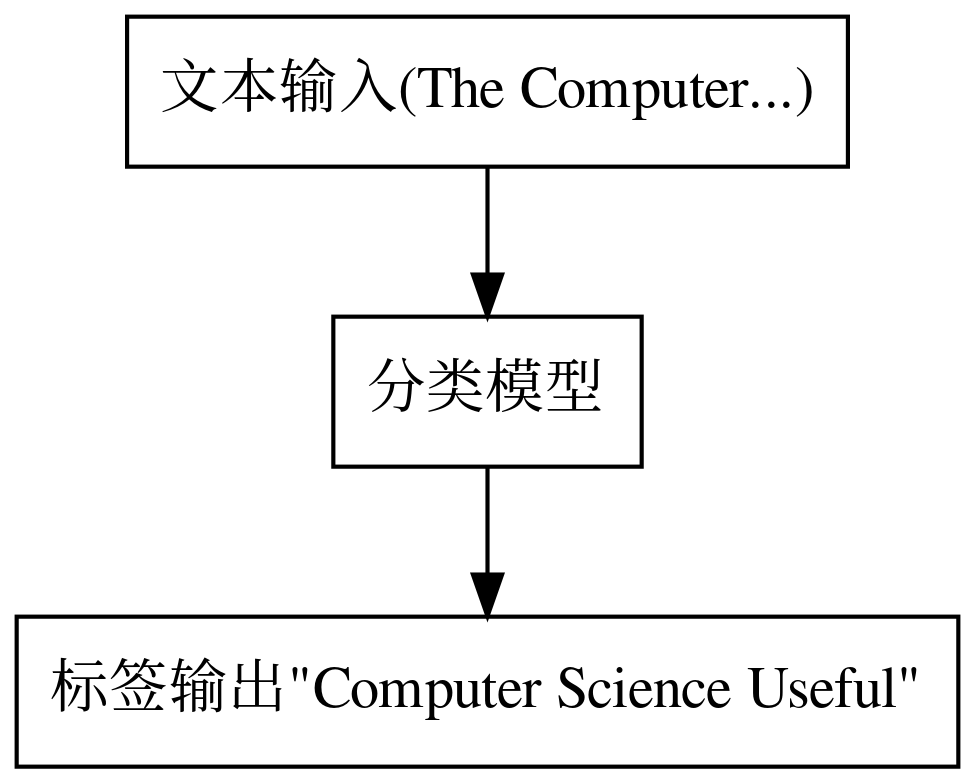
\includegraphics[width=5cm]{./figs/text-classification}
  \caption{文本分类}
  \label{fig:text-classification}
\end{figure}

\subsection{流程}
文本分类的一般化流程如图\ref{fig:textclassification}所示,首先获取到原始数据,通常可使用
API或爬虫。获取到原始数据后就要通常要先进行分词,本文采
用英文文本,分词较为简单,直接取空格分隔即可。分词后,须对每个词进行数据清洗和预处理,取出数字、标点等特殊符号,
去掉停用词、网址、超链接等。获取到“干净”的数据后,使用如TF-IDF、BOW、主题模型等方式对文本
进行特征表示,最后使用提取到的特征,进行分类算法的应用。

\begin{figure}[H]
  \centering
  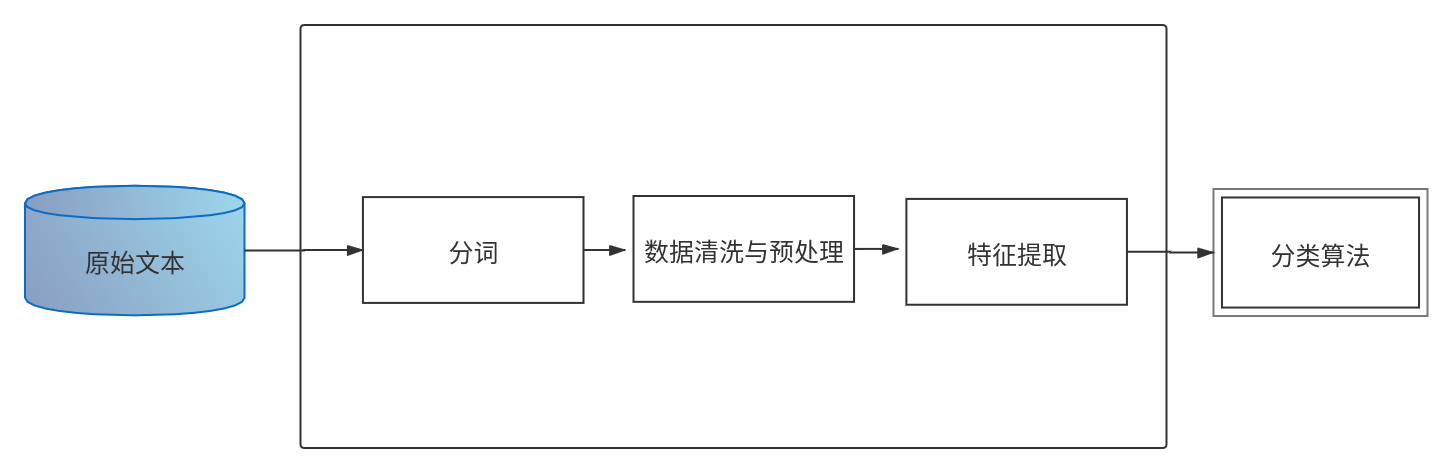
\includegraphics[width=1.0\textwidth]{process}
  \caption{文本分类的一般流程}
  \label{fig:textclassification}
\end{figure}

\section{有监督的短文本分类方法}

\subsection{短文本预处理}
文本预处理是信息检索和文本数据挖掘任务中的重要环节和关键性步骤。一般包括,文档分割、大小写转换
分词、词干提取、词形还原
、去除停用词、规范化、去噪等。

文档分割的步骤通常需要根据文本数据的形式来判断是否需要进行,如果数据集中的每篇文档没有过大且较
为独立,则不需要进行。反之,如果所有的或者大部分数据保存在一个文档中,即需要进行文档切割,
将其分成若干小份,方便后续处理。当然,若多篇文档处于同一个文件中,会有一些特殊的标记区分数
据块,在编程时也很方便去处理。

如果文本是英文字符,则需要将其统一为小写字母,可以降
低字典重复率。

分词,就是将一个句子分成一个个词汇的过程。目的是使得词变成最基础的“数据结
构”,方便后续处理。分词在某种意义上就可以看成是对问题的形式化,将“无结构”的文本数据,
整理成“结构化数据”,方便进行特征表示,分词是所有文本处理类问题形式化的第一步。

词干提取(steming),是将
词语中的变形减少到其“根”的形式的过程。例如将“connect”、“connectedy”以及“connection”都转化
成“connnect”。词干提取能够一定程度上缓解稀疏性问题,在搜索引擎中也常常会发现这个技术,比如
你在Google搜索“deeplearning course”和“deep learning course”,通常你都可以获得正确的结果,
就是因为搜索引擎做了这样的处理。词形还原(lemmatization),目标是删除变形并找到“根”形式。与
词干提取区别在于,词形还原寻找正确的词缀,而词干提取只是在相同的位置做切断。% 例如,
% “trouble”、“troubling”、“troubled”都词形还原会映射为“trouble”,而词干提取只会映射成“troubl”。
下面是词形还原和词形提取的对比图:

\begin{table}[H]                                                                    \begin{singlespace}                                                          
    \centering\caption{词干提取和词形还原对比}\label{tab:level}
    \renewcommand{\arraystretch}{1.5} %控制行高    
    \begin{tabular}{lll}\hline
      Original word & stemmed word & lemmatized word \\  \hline                                                
      \verb|trouble| & troubl & trouble\\                                                   
      \verb|troubling| & troubl &trouble \\                                                 
      \verb|troubled| & troubl & trouble \\                                                 
      \verb|troubles| & troubl & trouble \\
      \verb|troublesome| & troubl & trouble \\      
      \hline                                                                  
\end{tabular}                                                              
\end{singlespace}                                                            \end{table}               

停用词是一种语言中最常见的、无实际意义的词。例如,英文中的be动词、介词、连词等。去停用词的目的是删除文本中低信息量词对主题词的影响,使得算法对文本内容有更强的辨别性。例如:
\par\hspace{5em}\verb|"The Computer Science is a quite uesful subject."|\par

去停用词后,
\par\hspace{5em}\verb|"Computer Science useful subject"|\par

规范化,例如“\$100”可以表示成“one hundred dollars”,“2morrow”转化成“tomorrow”。去噪,
用于删除文本非正常文本中的字符,如符号和数字等特殊字符,他们会对文本分析产生干扰。例如
hashtag中开头的“\#”,提醒关注的“@”,超文本链接“https”,转发推文的“RT”等都是需要被处理的。% 最
% 后,文本增强,它是考虑使用外部语料库即之前不存在的消息来扩充文本数据,使得文本语义得到增强,
% 从而进一步提高模型的预测能力。

% subsection{语言模型}         
% 在介绍词向量的特征表示之前,我们需要先了解下语言模型。语言模型是统计学在自然语言处理上的应
% 用,它根据语言的上下文建立数学模型,描述当前词相对于整个文本的关系。N-gram模型是最常见
% 的一种语言模型,可以用来判断一个文档的出现是
% 否合理,也就是将文档出现的可能用概率表示出来。在该模型中,单词被映射到高维空间,然后嵌入组
% 合以获取输入句子的固定大小表示,后来用作输入到分类器。然而,由于考虑了短句中的词序,它容易
% 受到数据高维稀疏的影响。N-gram模型使用链式法则来计算文档出现的联合概率:
% \begin{equation}
%   \label{eq:1}                                                                              
% P(w_1,w_2,\ldots,w_n) = P(w_1)P(w_2\mid w_1)P(w_3\mid w_1,w_2) \ldots P(w_n \mid w_1, w_2,                                                                    
% \ldots, w_{n-1})                                                               
% \end{equation}

\subsection{词向量特征表示}
类似于图像像素点,对于计算机来说,文本字符实际上是无法直接被理解的。在解决文本分类问题时,
需先将文本转化成结构化的向量信息,才能继续应用算法进行处理。

最简单的特征表示方法就是词袋模型(Bag-of-Words)\cite{zhang2010understanding},它将所有的语料中出现的单词看成一个词汇表,词汇表的大
小即为向量空间的大小,文本中所有文档的维度都和该词汇表的维度相同,通过统计每个词出现的次数,
当作该词在向量中的权重。通俗的讲,就是将一篇文档看做是词的袋子,里面装着一个个不同的词。显
然,文档被转换为一个个词以后,词和词之间的上下文关系也就丢失了。

TF-IDF(Term Frequency–Inverse Document Frequency)\cite{ramos2003using},频率-逆文档频率,旨在反映单词对集合或语料库中的文档的重要程度。

TF(Term Frequency),表示某个单词出现的次数,即词频。其表达式如\ref{eq:tf}所示:

\begin{equation}
  \label{eq:tf}
  TF(t_i) = \frac{n_{i, j}}{\sum_k{n_{k,j}}}
\end{equation}

其中,$t_i$表示文本中的第$i$个单词,$n_{i,j}$表示该单词在第$j$个中文档中出现的次数,而分母
是整个语料中出现的所有词的出现次数之和。

IDF(Inverse Document Frequency,逆文档频率),是一个词语普遍重要性的度量,IDF的值越大,说
明该单词重要性越高,更具有代表性。某一单词的IDF值可以由总文本数除以包含该单词的文本数,再
对其得到的商求对数,其表达式如\ref{eq:idf}所示:

\begin{equation}
  \label{eq:idf}
  IDF(t_i) = lg{\frac{|D|}{|\{j:t_i \in d_j\}|}}
\end{equation}
其中,|D|为语料库中的文件总数,
$|\{j:t_i \in d_j\}|$包含词语$t_i$的文件数目,如果词语不在数据中,就导致分母为零,因此一
般情况下使用$1+|\{j:t_i \in d_j\}|$。
最后,得到TF-IDF:

\begin{equation}
  \label{eq:tf-idf}
  TF-IDF_{i,j} = TF_{i,j} × IDF_{i}
\end{equation}

TF-IDF本质上基于词袋模型。

 \subsection{主题模型}           
主题模型是一种基于概率的非监督聚类统计模型,它通过挖掘文档的隐含语义结构(Latent Semanmitc Structure)
,对文档进行分析。不同于传统的语言模型,只考虑文档在空间上的维度,而引入主题的概念,实现文
档在主题空间上的表示。主题模型在文本挖掘问题中的应用十分广泛,其中最著名的就是David Blei提
出的LDA(Latent Dirichlet Allocation)主题模型\cite{blei2003latent}。

LDA是一种生成模型,假设整个语料库一共包含K个主题,每个主题z都被表示成一个词典V上的一元语言模型$\vartheta_{z}$,即词典上的一个多项
式分布。我们进一步假设每个文档对于这个主题有一个文档特定的多项式$\varPhi_{d}$。那么,文档的生成
过程如图\ref{fig:lda}:

\begin{figure}[H]
  \centering
  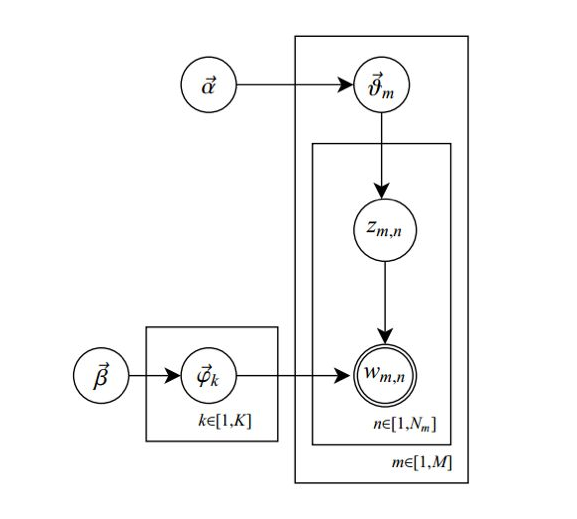
\includegraphics[width=10cm]{./figs/lda.png}
  \caption{LDA主题模型}
  \label{fig:lda}
\end{figure}

其中,$N_m$表示文档中词语的数量,M表示文档的总数量,K表示主题数,$\vartheta$表示文档与主题
之间的多项式分布,$\varphi$表示主题和主题词之间的多项式分布
,$\alpha$和$\beta$分别是$\vartheta$和$\varphi$的
Dirichlet先验参数,$Z_{m,n}$表示词语的主题分布,$w_{m,n}$表示生成的词。生成文档的步骤如下:
\begin{itemize}
\item 从参数为$\alpha$的Dirichlet分布中采样生成主题的多项式分布$\varphi$,
\item 从主题的多项式分布$\varphi$中采样生成第j个主题词$z_{i,j}$
\item 从参数为$\beta$的Dirichlet分布中采样生成主题$z_{i,j}$对应词语的多项式分布$\varphi_{k}$
\item 从词语的多项式分布$\varphi_{k}$中采样生成最终词语$w_{i,j}$
\end{itemize}

 % \subsection{文本扩展技术}
 % 常见的文本扩展技术有基于主题模型(Topic Model)的短文本扩展技术以及基于外部语料库的文本扩
 % 展技术。
 
\section{有监督的短文本数据流分类方法}
% 本小节将介绍有监督的短文本数据流分类方法,需要用到的基础理论和技术, 分别数据流定义、支持向
% 量机、集成分类方法 、相似性度量、分类效果衡量指标
% 以及概念漂移。

\subsection{数据流定义}
数据流是由随着时间推移到达的大量的、连续的数据项组成的序列\cite{陈火旺A}。若令t表示某一时刻,
则数据流可形式化地表示为$D=\{d_1,d_2,…,d_{t-1},d_{t},d_{t+1},…\}$其中,$d_t=\{x_{t},y_{t}\}$,
$x_{t}$为第i个属性值,$y_{t}$表示该属性值对应的类标签。

数据流具备动态实时、持续到达、易变、高维稀疏等特点。正是由于这些特点,使得数据流无法将传统的机器学习算法如决策树、支持向量机、贝叶斯等算法直接应用,这给数据流分析带来了挑战。

\subsection{支持向量机}
支持向量机(Support Vector machine),是一种有监督(Supervised Learning)
\cite{russell2002artificial} 的二元分类器。首次
由Vapnik等人1964年提出\cite{Vapnik1964A},而后又经过多次优化与提高,使其可以应用于多元分类
任务\cite{Hsu2002A}。其基
本模型定义为特征空间上的间隔最大的线性分类器,即在样本空间中找到一个超平面,使得它可以最大
分隔两个类。

\begin{figure}[H]
  \centering
  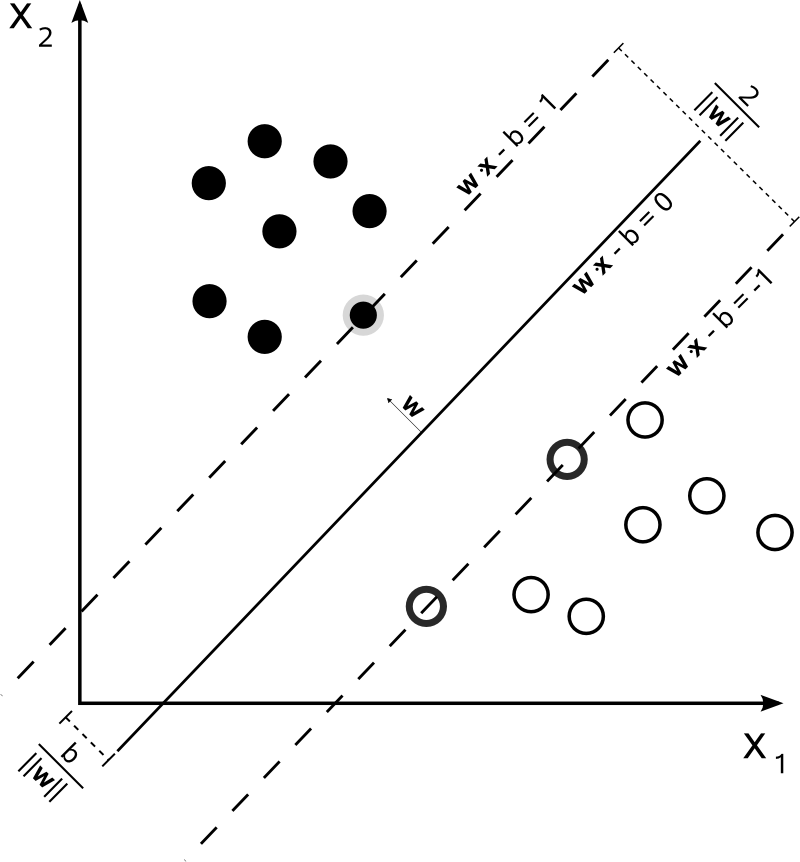
\includegraphics[width=10cm]{./figs/svm.png}
  \caption{支持向量机}
  \label{fig:svm}
\end{figure}

如图\ref{fig:svm}所示,其中$wx-b=1$和$wx-b=-1$表示两条支持向量,中间的$wx-b=0$即为找到的超
平面。对于这样一个二维数据集来说,最优超平面的寻找较为简单,但实际使用中的数据集往往远超二维,
对于这样的高维数据来说,不一定都是线性可分的,因此想要找到最佳超平面的就需要借助核函数,将样本空间映射到更高维的空间,
使得数据变得线性可分,以方便更好的进行样本分离。通常,核函数的选择也会直接影响到模型的分类性能,故如何选择更好的
核函数也很重要,下面是几种SVM常用的核函数:

\begin{table}[H]                                                                    \begin{singlespace}                                                          
    \centering\caption{SVM核函数对比}\label{tab:level}
    \renewcommand{\arraystretch}{1.5} %控制行高    
    \begin{tabular}{llp{6cm}}\hline
      核函数 & 计算公式 & 描述 \\  \hline                                                
      \verb|线性核函数| & $K(x_i,x_j)=x_i^Tx_j$ & 其中,K为半正定核矩阵,适用于线性可分的数据,速度较快\\                                                   
      \verb|多项式核函数| & $K(x_i,x_j)=(x_i^Tx_j)^d$ &  其中,$d \geq 1$\\
      \verb|高斯核函数| & $K(x_i,x_j)=exp(-\frac{{||x_i-x_j||}^2}{2\sigma^2})$ & 其中,$\sigma
                                                                                 \geq 0$
                                                                                 为高斯核
                                                                                 的带宽 \\
      \verb|拉普拉斯核函数| & $K(x_i,x_j)=exp(-\frac{||x_i-x_j||}{\sigma})$ & $\sigma
                                                                                 \geq 0$ \\
      \verb|Sigmoid 核函数| &  $K(x_i,x_j)=tanh(\beta x_i^Tx_j+\theta)$ & 其中, $tanh$为双曲正切函数,$\beta>0$,$\theta>0$ \\            
      \hline                                                                  
\end{tabular}                                                              
\end{singlespace}
\end{table}

\subsection{集成方法}
集成方法也叫集成学习(Ensemble Learning) ,不同于决策树、支持向量机等分类器的是,它不是一
个新的分类算法,而是一种机器学习范式。集成方法的思想是,通过训练多个分类模型,将所有的模型
综合起来得到更好的预测结果。大量的实践证明它能够带来更高的准确率和更强的鲁棒性。

在快速数据流中,分类模型通常不能稳健地建立。因此,采用集成分类方法,通过组合不同的分类器可
以使模型更加健壮。另一方面,数据以流的形式出现, 在机器的内存中直接容纳大量流数据是不切
实际的,而且通常是不可行的。因此在这种情况下,可以借助集成模型,连续更新并通过使用最近一批
数据进行再训练来增量地训练预测模型。bagging和boosting是两种最常见的集成方法\cite{oza2005online}。

Street等\cite{street2001streaming}将集成应用到文本数据流分类中,思想是以块为单位顺序读取训
练数据,在当前块学习分类器,并在下一个块上进行评估,缺点是没有考虑到概念漂移。wettschereck
等\cite{wettschereck2003mining}设计了处理概念漂移的集成方法,它可以有效地发现数据流的迁移,该方法中,数据流被分割成块,每个块上都有多个分类器,并且最终的分类权值通过每个块上函数计算。kotler,zhang等\cite{kotler2003dynamic,zhang2009mining}也都使用这种模型加权或模型选择方法,来确保概念漂移数据流分类获得更好的
精度。

\subsection{概念漂移}
概念漂移(Concept Drift)\cite{widmer1996learning} 是指在非平稳的环境中,数据分布会随着时
间而变化,改变数据流上下文中的隐含信息,从而产生概念漂移现象。数据流分类的目标是训练分类
器,建立一个类标签和特征之间的函数关系。而概念漂移是数据流分类中最早出现的,也是比较棘手的问题之一。
  
一个典型的示例是用户对新闻信息流兴趣的变化,虽然新闻文档的分发通常保
 持不变,但该用户感兴趣的新闻文档的条件分布却发生了变化。

最通用的解决思路就是通过历史数据分析,抽象出数                             据的模式随时间变化的规律,其中可能包括若干趋势和周期的混杂信号。但多数情况下,随时间的变化
有很强的随机性,这很难做到。

在过去的一段时间里,与概念漂移有关的学习的研究越来越多,并且已经开发了许多漂移感知的自适应学习算法。
自适应学习是指在运行过程中在线更新预测模型以对概念漂移做出
反应。Tsymbal等人在2004年发表的概念漂移综述文章\cite{tsymbal2004problem}对该问题给出了相对较全的定
义,并附出了当时相关工作;kuncheva\cite{kuncheva2004classifier,kuncheva2008classifier}将集
成学习技术应用于概念漂移检测上。maloof等提出了归纳规则学习算法\cite{maloof2010aq};
shirakawa等基于语
义扩展的方法\cite{shirakawa2015wikipedia}以及phan等基于主题模型的方法\cite{phan2010hidden}
下面将主要将描述自适应学习算法的特点。

自适应学习算法可以看作是先进的增量学习算法,能够随着时间的推移适应生成数据的过程。假设数据满足独立同分布,首先建立静态的基模型作为评估基准,默认随时间推移自变量和因变量的映
射关系一致,在通过这个模型检测是否存在概念漂移。
在训练之前,根据时序给样本不同的权重,时间越新的样
本权重可以给大一点,越老的数据可以减少权重                                      。
然后定期的加入新数据更新模型。在加入新数据的时候,也可以进一
步筛选出最适合的样本进行重新训练,得到更加适合的模型。

%\subsection{相似性度量}
%\subsection{分类效果衡量指标}

\section{平台开发相关技术}
本文处实现相关算法外,还构建了一个可视化的数据挖掘平台。本小节将介绍搭建数据挖掘平台需要用
到的Web相关技术,其中包括Django框架、MongoDB数据库和Echart可视化图标的相关介绍。
\subsection{Django框架}
Django 是一个高级的 Python 网络框架,通过自动化或简化Web开发的常见任务,快速开发安全和可维
护的网站。Django让代码编写者只需要专注于编写应用程序,网站开发中麻烦的部分已经被封装
完成,无需重新开发。
 Django开发的应用有如下几个优点
\begin{itemize}
\item 具有很好的完备性,几乎提供Web开发所需要的所有模块;
\item 可以构建几乎任何类型的后端,处理各种格式(HTML、JSON、XML)的数据;
\item 重视安全问题,例如常见的SQL注入、CSRF攻击等都有很好的防护;
\item 采用类MVT的设计原则,易于扩展性、可维护性高;
\item 灵活性高,采用Python编写,天生具备跨平台的能力;
\end{itemize}

Django的核心是一组高效协同工作的库,涵盖了Web开发的各个方面,其中包括:ORM对象关系映射器,该库知道数据库的结构,代码的结构,并且无需重复的手写SQL语句就能弥合它们之间的鸿沟。一组HTTP
库,它们知道如何解析传入的Web请求,并返回标准格式给用户。URL路由库,可让您准确定义所需的
URL并将它们映射到代码的适当位置。一个视图系统, 用于处理请求。 
Template模板系统,使用它编写混合模板语言的HTML代码,接受后端传来的数据,在网页中显示表单并
处理用户提交的数据。图\ref{fig:django}是Django的整体框架图。

\begin{figure}
  \centering
  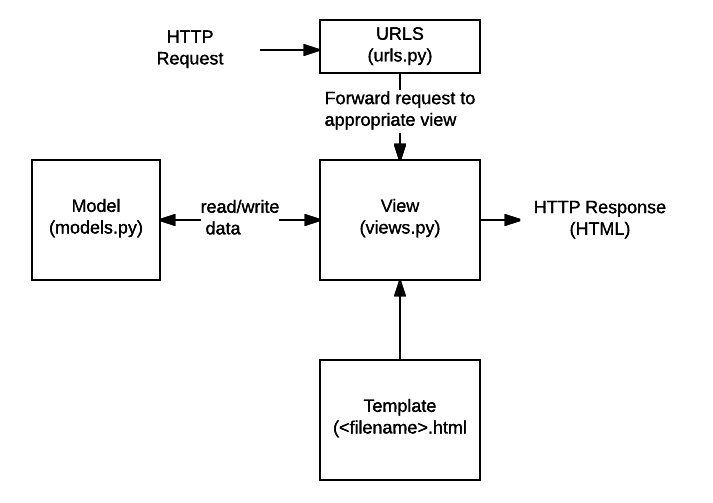
\includegraphics[width=10cm]{django}
  \caption{Django MVT设计框架图\cite{mozilla.org}}
  \label{fig:django}
\end{figure}

\subsection{MongoDB}
MongoDB是一种NoSQL数据库,NoSQL被称作“Not Only SQL”,在数据爆炸的今天使用十分广泛。
几年前,应用程序通常只拥有数千个用户到上万个用户,而现在流行的APP如“新浪微博”、
“Wechat”的用户都数以亿计,并且每年365天,每天7*24小时处于连接状态。传统的关系型数据库在处
理少量数据时它们具有良好的性能。但处理当下信息大爆炸时代互联网,多媒体和社交网络的海量数据,
使用传统的关系数据库效率低下。为了克服这个问题,引入了“ NO SQL”一词。 NoSQL术语由Carlo
Strozzi于1998年创造,指非关系数据库。MongoDB就是最流行的NoSQL数据库之一。

MongoDB采用C++语言编写的,一个开源的分布式文件存储数据库系统。MongoDB将所有的数据都是为文
档,文档数据结构表示方式采用Key-Value的形式,类似于JSON。

MongoDB主要特点如下:
\begin{itemize}
\item 可实现传统数据库能实现的所有操作;
\item 采用面向文档的设计模式,操作更加简单;
\item 由于存储特点,可应用于分布式计算;
\item 读取效率相比传统数据库更高;
\item 丰富的查询表达式。可轻易查询文档中内嵌的对象及数组;
\item 支持多种编程语言,安装便捷;

  图\ref{fig:mongodb}是MongoDB的架构:
  \begin{figure}
  \centering
  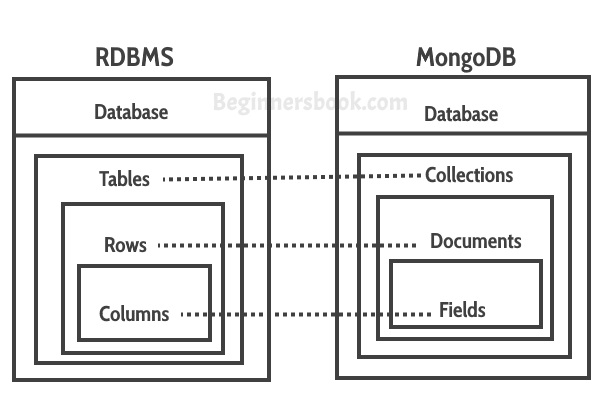
\includegraphics[width=10cm]{mongodb}
  \caption{RDBMS vs MongoDB\cite{beginnersbook.com}}
  \label{fig:mongodb}
\end{figure}
\end{itemize}

\subsection{Echart}
ECharts(Enterprise Charts)是国产的应用于浏览器的可视化工具箱。使用简单的Javascript语法,就可以完成对数据的操作,同时画出美观的图表。

\section{本章小结}
本章节详细介绍了本文研究问题相关的技术和理论,其中包括大数据分析的基本流程,讨论了文本分类常用
的技术手段。并对有监督的文本分类方法和有监督的文本数据流分类方法分别做了理论介绍,大致包括文本
预处理、语言模型、词特征表示、主题模型、数据流定义、支持向量机、集成分类方法、概念漂移现象
等。通过阅读本章节,读者可以对本文研究的背景知识有了大致的了解。
